% Copyright 2006 by Tilo Tantau
%
% This file may be distributed and/or modified
%
% 1. under the LaTeX Project Public License and/or
% 2. under the GNU Free Documentation License.
%
% See the file doc/generic/pgf/licenses/LICENSE for more details.

\section{Tutorial: A Petri-Net for Hagen}

In this second tutorial we explore the node mechanism of
\tikzname\ and \pgfname.

Hagen must give a talk tomorrow about his favorite formalism for
distributed systems: Petri nets! Hagen used to give his talks using a
blackboard and everyone seemed to be perfectly content with
this. Unfortunately, his audience has been spoiled recently with fancy
projector-based presentations and there seems to be a certain amount
of peer pressure that his Petri nets should also be drawn using a
graphic program. One of the professors at his institute recommends
\tikzname\ for this and Hagen decides to give it a try.


\subsection{Problem Statement}

For his talk, Hagen wishes to create a graphic that demonstrates how a
net with place capacities can be simulated by a net without
capacities. The graphic should look like this, ideally:

\begin{quote}
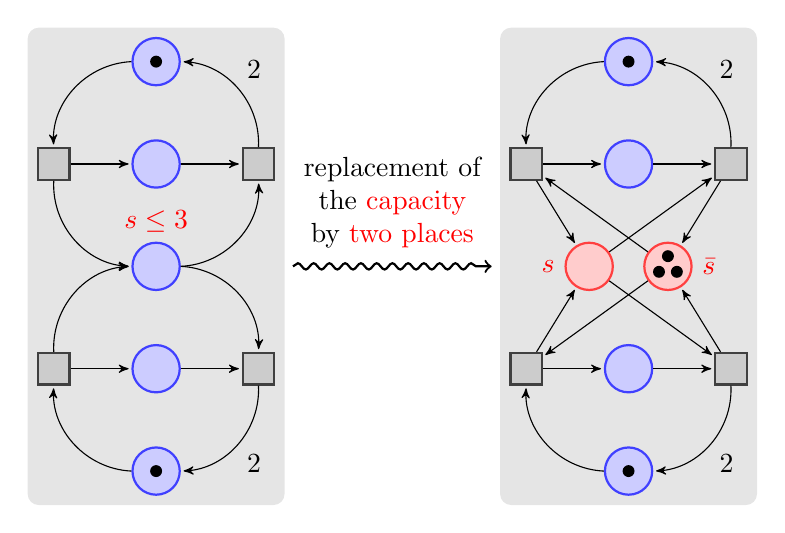
\begin{tikzpicture}
  [node distance=1.3cm,>=stealth',bend angle=45,auto,
   place/.style={circle,thick,draw=blue!75,fill=blue!20,minimum size=6mm},
   red place/.style={place,draw=red!75,fill=red!20},
   transition/.style={rectangle,thick,draw=black!75,fill=black!20,minimum size=4mm},
   every label/.style={red},on grid]

  \begin{scope}
    % First net
    \node [place,tokens=1] (w1)                                    {};
    \node [place] (c1) [below=of w1]                      {};
    \node [place] (s)  [below=of c1,label=above:$s\le 3$] {};
    \node [place] (c2) [below=of s]                       {};
    \node [place,tokens=1] (w2) [below=of c2]                      {};

    \node [transition] (e1) [left=of c1] {}
      edge [pre,bend left]                  (w1)
      edge [post,bend right]                (s)
      edge [post]                           (c1);

    \node [transition] (e2) [left=of c2] {}
      edge [pre,bend right]                 (w2)
      edge [post,bend left]                 (s)
      edge [post]                           (c2);

    \node [transition] (l1) [right=of c1] {}
      edge [pre]                            (c1)
      edge [pre,bend left]                  (s)
      edge [post,bend right] node[swap] {2} (w1);

    \node [transition] (l2) [right=of c2] {}
      edge [pre]                            (c2)
      edge [pre,bend right]                 (s)
      edge [post,bend left]  node {2}       (w2);
  \end{scope}

  \begin{scope}[xshift=6cm]
    % Second net
    \node [place,tokens=1]
                      (w1')                                                {};
    \node [place]     (c1') [below=of w1']                                 {};
    \node [red place] (s1') [below=of c1',xshift=-5mm,label=left:$s$]      {};
    \node [red place,tokens=3]
                      (s2') [below=of c1',xshift=5mm,label=right:$\bar s$] {};
    \node [place]     (c2') [below=of s1',xshift=5mm]                      {};
    \node [place,tokens=1]
                      (w2') [below=of c2']                                 {};

    \node [transition] (e1') [left=of c1'] {}
      edge [pre,bend left]                  (w1')
      edge [post]                           (s1')
      edge [pre]                            (s2')
      edge [post]                           (c1');

    \node [transition] (e2') [left=of c2'] {}
      edge [pre,bend right]                 (w2')
      edge [post]                           (s1')
      edge [pre]                            (s2')
      edge [post]                           (c2');

    \node [transition] (l1') [right=of c1'] {}
      edge [pre]                            (c1')
      edge [pre]                            (s1')
      edge [post]                           (s2')
      edge [post,bend right] node[swap] {2} (w1');

    \node [transition] (l2') [right=of c2'] {}
      edge [pre]                            (c2')
      edge [pre]                            (s1')
      edge [post]                           (s2')
      edge [post,bend left]  node {2}       (w2');
  \end{scope}

  \begin{scope}[on background layer]
    \node (r1) [fill=black!10,rounded corners,fit=(w1)(w2)(e1)(e2)(l1)(l2)] {};
    \node (r2) [fill=black!10,rounded corners,fit=(w1')(w2')(e1')(e2')(l1')(l2')] {};
  \end{scope}

  \draw [shorten >=1mm,-to,thick,decorate,decoration={snake,amplitude=.4mm,segment
      length=2mm,pre=moveto,pre length=1mm,post length=2mm}]
    (r1) -- (r2)
    node [above=1mm,midway,text width=3cm,align=center]
      {replacement of the \textcolor{red}{capacity} by \textcolor{red}{two places}};

\end{tikzpicture}
\end{quote}


\subsection{Setting up the Environment}

For the picture Hagen will need to load the \tikzname\ package as did
Karl in the previous tutorial. However, Hagen will also need to load
some additional  \emph{library packages} that Karl did not need. These
library packages contain additional definitions like extra arrow tips
that are typically not needed in a picture and that need to be
loaded explicitly.

Hagen will need to load several libraries: The |arrows| library for the
special arrow tip used in the graphic, the |decoration.pathmorphing|
library for the ``snaking line'' in the middle, the |backgrounds|
library for the two rectangular areas that are behind the two main
parts of the picture, the |fit| library to easily compute the sizes of
these rectangles, and the |positioning| library for placing nodes
relative to other nodes.


\subsubsection{Setting up the Environment in \LaTeX}

When using \LaTeX\ use:

\begin{codeexample}[code only]
\documentclass{article} % say

\usepackage{tikz}
\usetikzlibrary{arrows,decorations.pathmorphing,backgrounds,positioning,fit,petri}

\begin{document}
\begin{tikzpicture}
  \draw (0,0) -- (1,1);
\end{tikzpicture}
\end{document}
\end{codeexample}


\subsubsection{Setting up the Environment in Plain \TeX}

When using plain \TeX\ use:

\begin{codeexample}[code only]
%% Plain TeX file
\input tikz.tex
\usetikzlibrary{arrows,decorations.pathmorphing,backgrounds,positioning,fit,petri}
\baselineskip=12pt
\hsize=6.3truein
\vsize=8.7truein
\tikzpicture
  \draw (0,0) -- (1,1);
\endtikzpicture
\bye
\end{codeexample}


\subsubsection{Setting up the Environment in Con\TeX t}

When using Con\TeX\ use\footnote{Note that \pgfname/\tikzname{} is not
  supported by recent Con\TeX t versions (like mark IV, the
  Lua\TeX-aware part of Con\TeX t).}:
\begin{codeexample}[code only]
%% ConTeXt file
\usemodule[tikz]
\usetikzlibrary[arrows,decorations.pathmorphing,backgrounds,positioning,fit,petri]

\starttext
  \starttikzpicture
    \draw (0,0) -- (1,1);
  \stoptikzpicture
\stoptext
\end{codeexample}



\subsection{Introduction to Nodes}

In principle, we already know how to create the graphics that Hagen
desires (except perhaps for the snaked line, we will come to that): We
start with big light gray rectangle and then add lots of circles and
small rectangle, plus some arrows.

However, this approach has numerous disadvantages: First, it is hard
to change anything at a later stage. For example, if we decide to add
more places to the Petri nets (the circles are called places in Petri
net theory), all of the coordinates change and we need to recalculate
everything. Second, it is hard to read the code for the Petri net as it is just a long and complicated list of coordinates and drawing
commands -- the underlying structure of the Petri net is lost.

Fortunately, \tikzname\ offers a powerful mechanism for avoiding the
above problems: nodes. We already came across nodes in the previous
tutorial, where we used them to add labels to Karl's graphic. In the
present tutorial we will see that nodes are much more powerful.

A node is a small part of a picture. When a node is created, you
provide a position where the node should be drawn and a
\emph{shape}. A node of shape |circle| will be drawn as a circle, a
node of shape |rectangle| as a rectangle, and so on. A node may also
contain some text, which is why Karl used nodes to show text. Finally,
a node can get a \emph{name} for later reference.

In Hagen's picture we will use nodes for the places and for the
transitions of the Petri net (the places are the circles, the
transitions are the rectangles). Let us start with the upper half of
the left Petri net. In this upper half we have three places and two
transitions. Instead of drawing three circles and two rectangles, we
use three nodes of shape |circle| and two nodes of shape
|rectangle|.

\begin{codeexample}[]
\begin{tikzpicture}
  \path ( 0,2) node [shape=circle,draw] {}
        ( 0,1) node [shape=circle,draw] {}
        ( 0,0) node [shape=circle,draw] {}
        ( 1,1) node [shape=rectangle,draw] {}
        (-1,1) node [shape=rectangle,draw] {};
\end{tikzpicture}
\end{codeexample}

Hagen notes that this does not quite look like the final picture, but
it seems like a good first step.

Let us have a more detailed look at the code. The whole picture
consists of a single path. Ignoring the |node| operations, there is not
much going on in this path: It is just a sequence of coordinates with
nothing ``happening'' between them. Indeed, even if something were to
happen like a line-to or a curve-to, the |\path| command would not
``do'' anything with the resulting path. So, all the magic must be in
the |node| commands.

In the previous tutorial we learned that a |node| will add a piece of
text at the last coordinate. Thus, each of the five nodes is added at
a different position. In the above code, this text is empty
(because of the empty |{}|). So, why do we see anything at all? The
answer is the |draw| option for the |node| operation: It causes the
``shape around the text'' to be drawn.

So, the code |(0,2) node [shape=circle,draw] {}| means the following:
``In the main path, add a move-to to the coordinate |(0,2)|. Then,
temporarily suspend the construction of the main path while the node
is built. This node will be a |circle| around an empty text. This
circle is to be |draw|n, but not filled or otherwise used. Once this
whole node is constructed, it is saved until after the
main path is finished. Then, it is drawn.'' The following
|(0,1) node [shape=circle,draw] {}| then has the following effect:
``Continue the main path with a move-to to |(0,1)|. Then construct a
node at this position also. This node is also shown after the main
path is finished.'' And so on.



\subsection{Placing Nodes Using the At Syntax}

Hagen now understands how the |node| operation adds nodes to the path,
but it seems a bit silly to create a path using the |\path| operation,
consisting of numerous superfluous move-to operations, only to place
nodes. He is pleased to learn that there are ways to add nodes in a
more sensible manner.

First, the |node| operation allows one to add
|at (|\meta{coordinate}|)| in order to directly specify where the node
should be placed, sidestepping the rule that nodes are placed on the
last coordinate. Hagen can then write the following:

\begin{codeexample}[]
\begin{tikzpicture}
  \path node at ( 0,2) [shape=circle,draw] {}
        node at ( 0,1) [shape=circle,draw] {}
        node at ( 0,0) [shape=circle,draw] {}
        node at ( 1,1) [shape=rectangle,draw] {}
        node at (-1,1) [shape=rectangle,draw] {};
\end{tikzpicture}
\end{codeexample}

Now Hagen is still left with a single empty path, but at least the
path no longer contains strange move-tos. It turns out that this can
be improved further: The |\node| command is an abbreviation for
|\path node|, which allows Hagen to write:

\begin{codeexample}[]
\begin{tikzpicture}
  \node at ( 0,2) [circle,draw] {};
  \node at ( 0,1) [circle,draw] {};
  \node at ( 0,0) [circle,draw] {};
  \node at ( 1,1) [rectangle,draw] {};
  \node at (-1,1) [rectangle,draw] {};
\end{tikzpicture}
\end{codeexample}

Hagen likes this syntax much better than the previous one. Note that
Hagen has also omitted the |shape=| since, like |color=|, \tikzname\
allows you to omit the |shape=| if there is no confusion.



\subsection{Using Styles}

Feeling adventurous, Hagen tries to make the nodes look nicer. In the
final picture, the circles and rectangle should be filled with
different colors, resulting in the following code:

\begin{codeexample}[]
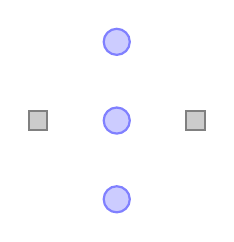
\begin{tikzpicture}[thick]
  \node at ( 0,2) [circle,draw=blue!50,fill=blue!20] {};
  \node at ( 0,1) [circle,draw=blue!50,fill=blue!20] {};
  \node at ( 0,0) [circle,draw=blue!50,fill=blue!20] {};
  \node at ( 1,1) [rectangle,draw=black!50,fill=black!20] {};
  \node at (-1,1) [rectangle,draw=black!50,fill=black!20] {};
\end{tikzpicture}
\end{codeexample}

While this looks nicer in the picture, the code starts to get a bit
ugly. Ideally, we would like our code to transport the message ``there
are three places and two transitions'' and not so much which
filling colors should be used.

To solve this problem, Hagen uses styles. He defines a style for
places and another style for transitions:

\begin{codeexample}[]
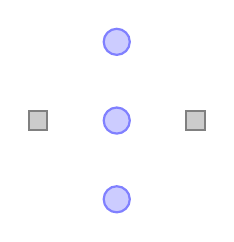
\begin{tikzpicture}
  [place/.style={circle,draw=blue!50,fill=blue!20,thick},
   transition/.style={rectangle,draw=black!50,fill=black!20,thick}]
  \node at ( 0,2) [place] {};
  \node at ( 0,1) [place] {};
  \node at ( 0,0) [place] {};
  \node at ( 1,1) [transition] {};
  \node at (-1,1) [transition] {};
\end{tikzpicture}
\end{codeexample}


\subsection{Node Size}

Before Hagen starts naming and connecting the nodes, let us first
make sure that the nodes get their final appearance. They are still
too small. Indeed, Hagen wonders why they have any size at all, after
all, the text is empty. The reason is that \tikzname\ automatically
adds some space around the text. The amount is set using the option
|inner sep|. So, to increase the size of the nodes, Hagen could write:

\begin{codeexample}[]
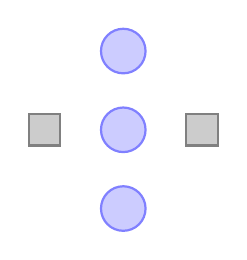
\begin{tikzpicture}
  [inner sep=2mm,
   place/.style={circle,draw=blue!50,fill=blue!20,thick},
   transition/.style={rectangle,draw=black!50,fill=black!20,thick}]
  \node at ( 0,2) [place] {};
  \node at ( 0,1) [place] {};
  \node at ( 0,0) [place] {};
  \node at ( 1,1) [transition] {};
  \node at (-1,1) [transition] {};
\end{tikzpicture}
\end{codeexample}

However, this is not really the best way to achieve the desired
effect. It is much better to use the |minimum size| option
instead. This option allows Hagen to specify a minimum size that the
node should have. If the node actually needs to be bigger because of
a longer text, it will be larger, but if the text is empty, then the
node will have |minimum size|. This option is also useful to ensure
that several nodes containing different amounts of text have the same
size. The options |minimum height| and |minimum width| allow you to
specify the minimum height and width independently.

So, what Hagen needs to do is to provide |minimum size| for the
nodes. To be on the safe side, he also sets |inner sep=0pt|. This
ensures that the nodes will really have size |minimum size| and not,
for very small minimum sizes, the minimal size necessary to encompass
the automatically added space.

\begin{codeexample}[]
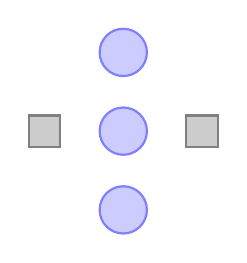
\begin{tikzpicture}
  [place/.style={circle,draw=blue!50,fill=blue!20,thick,
                 inner sep=0pt,minimum size=6mm},
   transition/.style={rectangle,draw=black!50,fill=black!20,thick,
                      inner sep=0pt,minimum size=4mm}]
  \node at ( 0,2) [place] {};
  \node at ( 0,1) [place] {};
  \node at ( 0,0) [place] {};
  \node at ( 1,1) [transition] {};
  \node at (-1,1) [transition] {};
\end{tikzpicture}
\end{codeexample}




\subsection{Naming Nodes}

Hagen's next aim is to connect the nodes using arrows. This seems like
a tricky business since the arrows should not start in the middle of
the nodes, but somewhere on the border and Hagen would very much like
to avoid computing these positions by hand.

Fortunately, \pgfname\ will perform all the necessary calculations for
him. However, he first has to assign names to the nodes so that he can
reference them later on.

There are two ways to name a node. The first is to use the |name=|
option. The second method is to write the desired name in parentheses
after the |node| operation. Hagen thinks that this second method seems
strange, but he will soon change his opinion.

{
\tikzset{place/.style={circle,draw=blue!50,fill=blue!20,thick,
                   inner sep=0pt,minimum size=6mm},
transition/.style={rectangle,draw=black!50,fill=black!20,thick,
                        inner sep=0pt,minimum size=4mm}}
\begin{codeexample}[]
% ... set up styles
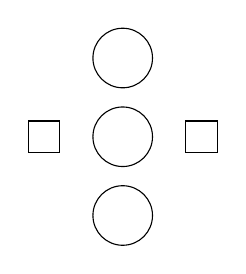
\begin{tikzpicture}
  \node (waiting 1)  at ( 0,2)     [place] {};
  \node (critical 1) at ( 0,1)     [place] {};
  \node (semaphore)  at ( 0,0)     [place] {};
  \node (leave critical) at ( 1,1) [transition] {};
  \node (enter critical) at (-1,1) [transition] {};
\end{tikzpicture}
\end{codeexample}
}

Hagen is pleased to note that the names help in understanding the
code. Names for nodes can be pretty arbitrary, but they should not
contain commas, periods, parentheses, colons, and some other special
characters. However, they can contain underscores and hyphens.

The syntax for the |node| operation is quite liberal with respect to
the order in which node names, the |at| specifier, and the options
must come. Indeed, you can even have multiple option blocks between
the |node| and the text in curly braces, they accumulate. You can
rearrange them arbitrarily and perhaps the following might be preferable:

{
\tikzset{place/.style={circle,draw=blue!50,fill=blue!20,thick,
                   inner sep=0pt,minimum size=6mm},
transition/.style={rectangle,draw=black!50,fill=black!20,thick,
                        inner sep=0pt,minimum size=4mm}}
\begin{codeexample}[]
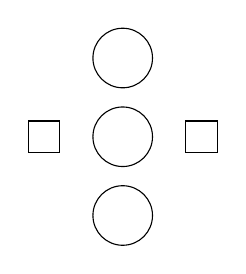
\begin{tikzpicture}
  \node[place]      (waiting 1)      at ( 0,2) {};
  \node[place]      (critical 1)     at ( 0,1) {};
  \node[place]      (semaphore)      at ( 0,0) {};
  \node[transition] (leave critical) at ( 1,1) {};
  \node[transition] (enter critical) at (-1,1) {};
\end{tikzpicture}
\end{codeexample}
}



\subsection{Placing Nodes Using Relative Placement}

Although Hagen still wishes to connect the nodes, he first wishes to
address another problem again: The placement of the nodes. Although he
likes the |at| syntax, in this particular case he would prefer placing
the nodes ``relative to each other.'' So, Hagen would like to say that
the |critical 1| node should be below the |waiting 1| node, wherever
the |waiting 1| node might be. There are different ways of achieving
this, but the nicest one in Hagen's case is the |below| option:

{
\tikzset{place/.style={circle,draw=blue!50,fill=blue!20,thick,
                   inner sep=0pt,minimum size=6mm},
transition/.style={rectangle,draw=black!50,fill=black!20,thick,
                        inner sep=0pt,minimum size=4mm}}
\begin{codeexample}[]
\begin{tikzpicture}
  \node[place]      (waiting)                            {};
  \node[place]      (critical)       [below=of waiting]  {};
  \node[place]      (semaphore)      [below=of critical] {};
  \node[transition] (leave critical) [right=of critical] {};
  \node[transition] (enter critical) [left=of critical]  {};
\end{tikzpicture}
\end{codeexample}
}

With the |positioning| library loaded, when an option like |below|
is followed by |of|, then the position of the node is shifted in
such a manner that it is placed at the distance |node distance| in the
specified direction of the given direction. The |node distance| is
either the distance between the centers of the nodes (when the
|on grid| option is set to true) or the distance between the borders
(when the |on grid| option is set to false, which is the default).

Even though the above code has the same effect as the earlier code, Hagen
can pass it to his colleagues who will be able to just read and
understand it, perhaps without even having to see the picture.



\subsection{Adding Labels Next to Nodes}

Before we have a look at how Hagen can connect the nodes, let us add
the capacity ``$s \le 3$'' to the bottom node. For this, two
approaches are possible:
\begin{enumerate}
\item Hagen can just add a new node above the |north| anchor of the
  |semaphore| node.
{
\tikzset{place/.style={circle,draw=blue!50,fill=blue!20,thick,
                   inner sep=0pt,minimum size=6mm},
transition/.style={rectangle,draw=black!50,fill=black!20,thick,
                        inner sep=0pt,minimum size=4mm}}
\begin{codeexample}[]
\begin{tikzpicture}
  \node[place]      (waiting)                            {};
  \node[place]      (critical)       [below=of waiting]  {};
  \node[place]      (semaphore)      [below=of critical] {};
  \node[transition] (leave critical) [right=of critical] {};
  \node[transition] (enter critical) [left=of critical]  {};

  \node [red,above] at (semaphore.north) {$s\le 3$};
\end{tikzpicture}
\end{codeexample}
}
This is a general approach that will ``always work.''

\item Hagen can use the special |label| option. This option is given
  to a |node| and it causes \emph{another} node to be added next to
  the node where the option is given. Here is the idea: When we
  construct the |semaphore| node, we wish to indicate that we want
  another node with the capacity above it. For this, we use the option
  |label=above:$s\le 3$|. This option is interpreted as follows: We
  want a node above the |semaphore| node and this node should read
  ``$s \le 3$.'' Instead of |above| we could also use things like
  |below left| before the colon or a number like |60|.
{
\tikzset{place/.style={circle,draw=blue!50,fill=blue!20,thick,
                   inner sep=0pt,minimum size=6mm},
transition/.style={rectangle,draw=black!50,fill=black!20,thick,
                        inner sep=0pt,minimum size=4mm}}
\begin{codeexample}[]
\begin{tikzpicture}
  \node[place]      (waiting)                            {};
  \node[place]      (critical)       [below=of waiting]  {};
  \node[place]      (semaphore)      [below=of critical,
                                      label=above:$s\le3$] {};
  \node[transition] (leave critical) [right=of critical] {};
  \node[transition] (enter critical) [left=of critical]  {};
\end{tikzpicture}
\end{codeexample}
}
  It is also possible to give multiple |label| options, this causes
  multiple labels to be drawn.
\begin{codeexample}[]
\tikz
  \node [circle,draw,label=60:$60^\circ$,label=below:$-90^\circ$] {my circle};
\end{codeexample}
  Hagen is not fully satisfied with the |label| option since the label
  is not red. To achieve this, he has two options: First, he can
  redefine the |every label| style. Second, he can add options to the
  label's node. These options are given following the |label=|, so he
  would write |label=[red]above:$s\le3$|. However, this does not quite
  work since \TeX\ thinks that the |]| closes the whole option list of
  the |semaphore| node. So, Hagen has to add braces and writes
  |label={[red]above:$s\le3$}|. Since this looks a bit ugly, Hagen
  decides to redefine the |every label| style.
{
\tikzset{place/.style={circle,draw=blue!50,fill=blue!20,thick,
                   inner sep=0pt,minimum size=6mm},
transition/.style={rectangle,draw=black!50,fill=black!20,thick,
                        inner sep=0pt,minimum size=4mm}}
\begin{codeexample}[]
\begin{tikzpicture}[every label/.style={red}]
  \node[place]      (waiting)                            {};
  \node[place]      (critical)       [below=of waiting]  {};
  \node[place]      (semaphore)      [below=of critical,
                                      label=above:$s\le3$] {};
  \node[transition] (leave critical) [right=of critical] {};
  \node[transition] (enter critical) [left=of critical]  {};
\end{tikzpicture}
\end{codeexample}
}
\end{enumerate}



\subsection{Connecting Nodes}

It is now high time to connect the nodes. Let us start with something
simple, namely with the straight line from |enter critical| to
|critical|. We want this line to start at the right side of
|enter critical| and to end at the left side of |critical|. For
this, we can use the \emph{anchors} of the nodes. Every node defines a
whole bunch of anchors that lie on its border or inside it. For
example, the |center| anchor is at the center of the node, the |west|
anchor is on the left of the node, and so on. To access the coordinate
of a node, we use a coordinate that contains the node's name followed
by a dot, followed by the anchor's name:

{
\tikzset{place/.style={circle,draw=blue!50,fill=blue!20,thick,
                   inner sep=0pt,minimum size=6mm},
transition/.style={rectangle,draw=black!50,fill=black!20,thick,
                        inner sep=0pt,minimum size=4mm}}
\begin{codeexample}[]
\begin{tikzpicture}
  \node[place]      (waiting)                            {};
  \node[place]      (critical)       [below=of waiting]  {};
  \node[place]      (semaphore)      [below=of critical] {};
  \node[transition] (leave critical) [right=of critical] {};
  \node[transition] (enter critical) [left=of critical]  {};
  \draw [->] (critical.west) -- (enter critical.east);
\end{tikzpicture}
\end{codeexample}
}

Next, let us tackle the curve from |waiting| to |enter critical|. This
can be specified using curves and controls:

{
\tikzset{place/.style={circle,draw=blue!50,fill=blue!20,thick,
                   inner sep=0pt,minimum size=6mm},
transition/.style={rectangle,draw=black!50,fill=black!20,thick,
                        inner sep=0pt,minimum size=4mm}}
\begin{codeexample}[]
\begin{tikzpicture}
  \node[place]      (waiting)                            {};
  \node[place]      (critical)       [below=of waiting]  {};
  \node[place]      (semaphore)      [below=of critical] {};
  \node[transition] (leave critical) [right=of critical] {};
  \node[transition] (enter critical) [left=of critical]  {};
  \draw [->] (enter critical.east) -- (critical.west);
  \draw [->] (waiting.west) .. controls +(left:5mm) and +(up:5mm)
                            .. (enter critical.north);
\end{tikzpicture}
\end{codeexample}
}

Hagen sees how he can now add all his edges, but the whole process
seems a but awkward and not very flexible. Again, the code seems to
obscure the structure of the graphic rather than showing it.

So, let us start improving the code for the edges. First, Hagen can
leave out the anchors:

{
\tikzset{place/.style={circle,draw=blue!50,fill=blue!20,thick,
                   inner sep=0pt,minimum size=6mm},
transition/.style={rectangle,draw=black!50,fill=black!20,thick,
                        inner sep=0pt,minimum size=4mm}}
\begin{codeexample}[]
\begin{tikzpicture}
  \node[place]      (waiting)                            {};
  \node[place]      (critical)       [below=of waiting]  {};
  \node[place]      (semaphore)      [below=of critical] {};
  \node[transition] (leave critical) [right=of critical] {};
  \node[transition] (enter critical) [left=of critical]  {};
  \draw [->] (enter critical) -- (critical);
  \draw [->] (waiting) .. controls +(left:8mm) and +(up:8mm)
                       .. (enter critical);
\end{tikzpicture}
\end{codeexample}
}

Hagen is a bit surprised that this works. After all, how did
\tikzname\ know that the line from |enter critical| to |critical|
should actually start on the borders? Whenever \tikzname\ encounters a
whole node name as a ``coordinate,'' it tries to ``be smart'' about
the anchor that it should choose for this node. Depending on what
happens next, \tikzname\ will choose an anchor that lies on the border
of the node on a line to the next coordinate or control point. The
exact rules are a bit complex, but the chosen point will usually be
correct -- and when it is not, Hagen can still specify the desired
anchor by hand.

Hagen would now like to simplify the curve operation somehow. It turns
out that this can be accomplished using a special path operation: the
|to| operation. This operation takes many options (you can even define
new ones yourself). One pair of options is useful for Hagen: The pair
|in| and |out|. These options take angles at which a curve should
leave or reach the start or target coordinates. Without these options,
a straight line is drawn:

{
\tikzset{place/.style={circle,draw=blue!50,fill=blue!20,thick,
                   inner sep=0pt,minimum size=6mm},
transition/.style={rectangle,draw=black!50,fill=black!20,thick,
                        inner sep=0pt,minimum size=4mm}}
\begin{codeexample}[]
\begin{tikzpicture}
  \node[place]      (waiting)                            {};
  \node[place]      (critical)       [below=of waiting]  {};
  \node[place]      (semaphore)      [below=of critical] {};
  \node[transition] (leave critical) [right=of critical] {};
  \node[transition] (enter critical) [left=of critical]  {};
  \draw [->] (enter critical) to                 (critical);
  \draw [->] (waiting)        to [out=180,in=90] (enter critical);
\end{tikzpicture}
\end{codeexample}
}

There is another option for the |to| operation, that is even better
suited to Hagen's problem: The |bend right| option. This option also
takes an angle, but this angle only specifies the angle by which the
curve is bent to the right:

{
\tikzset{place/.style={circle,draw=blue!50,fill=blue!20,thick,
                   inner sep=0pt,minimum size=6mm},
transition/.style={rectangle,draw=black!50,fill=black!20,thick,
                        inner sep=0pt,minimum size=4mm}}
\begin{codeexample}[]
\begin{tikzpicture}
  \node[place]      (waiting)                            {};
  \node[place]      (critical)       [below=of waiting]  {};
  \node[place]      (semaphore)      [below=of critical] {};
  \node[transition] (leave critical) [right=of critical] {};
  \node[transition] (enter critical) [left=of critical]  {};
  \draw [->] (enter critical) to                 (critical);
  \draw [->] (waiting)        to [bend right=45] (enter critical);
  \draw [->] (enter critical) to [bend right=45] (semaphore);
\end{tikzpicture}
\end{codeexample}
}

It is now time for Hagen to learn about yet another way of specifying
edges: Using the |edge| path operation. This operation is very similar
to the |to| operation, but there is one important difference: Like a
node the edge generated by the |edge| operation is not part of the
main path, but is added only later. This may not seem very important,
but it has some nice consequences. For example, every edge can have
its own arrow tips and its own color and so on and, still, all the
edges can be given on the same path. This allows Hagen to write the
following:


{
\tikzset{place/.style={circle,draw=blue!50,fill=blue!20,thick,
                   inner sep=0pt,minimum size=6mm},
transition/.style={rectangle,draw=black!50,fill=black!20,thick,
                        inner sep=0pt,minimum size=4mm}}
\begin{codeexample}[]
\begin{tikzpicture}
  \node[place]      (waiting)                            {};
  \node[place]      (critical)       [below=of waiting]  {};
  \node[place]      (semaphore)      [below=of critical] {};
  \node[transition] (leave critical) [right=of critical] {};
  \node[transition] (enter critical) [left=of critical]  {}
    edge [->]               (critical)
    edge [<-,bend left=45]  (waiting)
    edge [->,bend right=45] (semaphore);
\end{tikzpicture}
\end{codeexample}
}

Each |edge| caused a new path to be constructed, consisting of a |to|
between the node |enter critical| and the node following the |edge|
command.

The finishing touch is to introduce two styles |pre| and |post| and to
use the |bend angle=45| option to set the bend angle once and for all:

{
\tikzset{place/.style={circle,draw=blue!50,fill=blue!20,thick,
                   inner sep=0pt,minimum size=6mm},
transition/.style={rectangle,draw=black!50,fill=black!20,thick,
                        inner sep=0pt,minimum size=4mm}}
\begin{codeexample}[]
% Styles place and transition as before
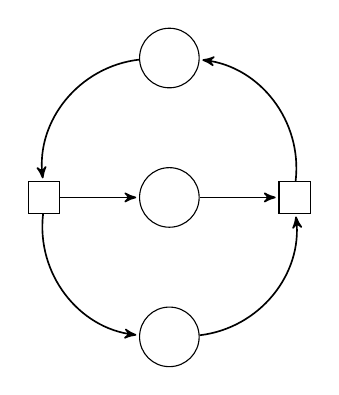
\begin{tikzpicture}
  [bend angle=45,
   pre/.style={<-,shorten <=1pt,>=stealth',semithick},
   post/.style={->,shorten >=1pt,>=stealth',semithick}]

  \node[place]      (waiting)                            {};
  \node[place]      (critical)       [below=of waiting]  {};
  \node[place]      (semaphore)      [below=of critical] {};

  \node[transition] (leave critical) [right=of critical] {}
    edge [pre]             (critical)
    edge [post,bend right] (waiting)
    edge [pre, bend left]  (semaphore);
  \node[transition] (enter critical) [left=of critical]  {}
    edge [post]            (critical)
    edge [pre, bend left]  (waiting)
    edge [post,bend right] (semaphore);
\end{tikzpicture}
\end{codeexample}
}




\subsection{Adding Labels Next to Lines}

The next thing that Hagen needs to add is the ``$2$'' at the arcs. For
this Hagen can use \tikzname's automatic node placement: By adding the
option |auto|, \tikzname\ will position nodes on curves and lines in
such a way that they are not on the curve but next to it. Adding
|swap| will mirror the label with respect to the line. Here is a
general example:

{
\begin{codeexample}[]
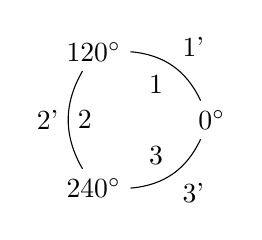
\begin{tikzpicture}[auto,bend right]
  \node (a) at (0:1) {$0^\circ$};
  \node (b) at (120:1) {$120^\circ$};
  \node (c) at (240:1) {$240^\circ$};

  \draw (a) to node {1} node [swap] {1'} (b)
        (b) to node {2} node [swap] {2'} (c)
        (c) to node {3} node [swap] {3'} (a);
\end{tikzpicture}
\end{codeexample}
}

What is happening here? The nodes are given somehow inside the |to|
operation! When this is done, the node is placed on the middle of the
curve or line created by the |to| operation. The |auto| option then
causes the node to be moved in such a way that it does not lie on the
curve, but next to it. In the example we provide even two nodes on
each |to| operation.

For Hagen that |auto| option is not really necessary since the two
``2'' labels could also easily be placed ``by hand.'' However, in a
complicated plot with numerous edges automatic placement can be a
blessing.

{
\tikzset{place/.style={circle,draw=blue!50,fill=blue!20,thick,
                   inner sep=0pt,minimum size=6mm},
transition/.style={rectangle,draw=black!50,fill=black!20,thick,
                        inner sep=0pt,minimum size=4mm},
pre/.style={<-,shorten <=1pt,>=stealth',semithick},
post/.style={->,shorten >=1pt,>=stealth',semithick}}
\begin{codeexample}[]
% Styles as before
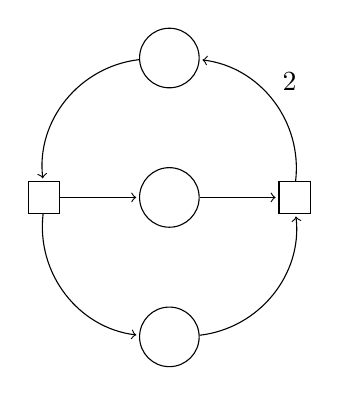
\begin{tikzpicture}[bend angle=45]
  \node[place]      (waiting)                            {};
  \node[place]      (critical)       [below=of waiting]  {};
  \node[place]      (semaphore)      [below=of critical] {};

  \node[transition] (leave critical) [right=of critical] {}
    edge [pre]                                 (critical)
    edge [post,bend right] node[auto,swap] {2} (waiting)
    edge [pre, bend left]                      (semaphore);
  \node[transition] (enter critical) [left=of critical]  {}
    edge [post]                                (critical)
    edge [pre, bend left]                      (waiting)
    edge [post,bend right]                     (semaphore);
\end{tikzpicture}
\end{codeexample}
}



\subsection{Adding the Snaked Line and Multi-Line Text}

With the node mechanism Hagen can now easily create the two Petri
nets. What he is unsure of is how he can create the snaked line
between the nets.

For this he can use a \emph{decoration}.
To draw the snaked line, Hagen only needs to set the two options
|decoration=snake| and |decorate| on
the path. This causes all lines of the path to be replaced by
snakes. It is also possible to use snakes only in certain parts of a
path, but Hagen will not need this.

\begin{codeexample}[]
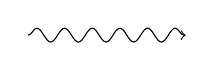
\begin{tikzpicture}
  \draw [->,decorate,decoration=snake] (0,0) -- (2,0);
\end{tikzpicture}
\end{codeexample}

Well, that does not look quite right, yet. The problem is that the
snake happens to end exactly at the position where the arrow
begins. Fortunately, there is an option that helps here. Also, the
snake should be a bit smaller, which can be influenced by even more
options.

\begin{codeexample}[]
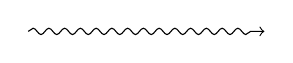
\begin{tikzpicture}
  \draw [->,decorate,
     decoration={snake,amplitude=.4mm,segment length=2mm,post length=1mm}]
    (0,0) -- (3,0);
\end{tikzpicture}
\end{codeexample}

Now Hagen needs to add the text above the snake. This text is a bit
challenging since it is a multi-line text. Hagen has two options for
this: First, he can specify an |align=center| and then use the |\\|
command to enforce the line breaks at the desired positions.

\begin{codeexample}[]
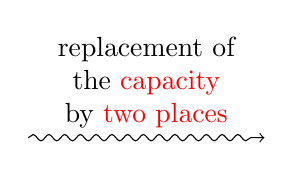
\begin{tikzpicture}
  \draw [->,decorate,
      decoration={snake,amplitude=.4mm,segment length=2mm,post length=1mm}]
    (0,0) -- (3,0)
    node [above,align=center,midway]
    {
      replacement of\\
      the \textcolor{red}{capacity}\\
      by \textcolor{red}{two places}
    };
\end{tikzpicture}
\end{codeexample}

Instead of specifying the line breaks ``by hand,'' Hagen can also
specify a width for the text and let \TeX\ perform the line breaking
for him:

\begin{codeexample}[]
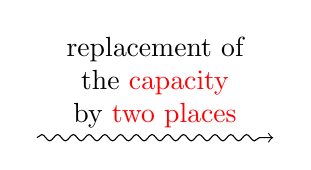
\begin{tikzpicture}
  \draw [->,decorate,
      decoration={snake,amplitude=.4mm,segment length=2mm,post length=1mm}]
    (0,0) -- (3,0)
    node [above,text width=3cm,align=center,midway]
    {
      replacement of the \textcolor{red}{capacity} by
      \textcolor{red}{two places}
    };
\end{tikzpicture}
\end{codeexample}



\subsection{Using Layers: The Background Rectangles}

Hagen still needs to add the background rectangles. These are a bit
tricky: Hagen would like to draw the rectangles \emph{after} the Petri
nets are finished. The reason is that only then can he conveniently
refer to the coordinates that make up the corners of the
rectangle. If Hagen draws the rectangle first, then he needs to know
the exact size of the Petri net -- which he does not.

The solution is to use \emph{layers}. When the background library is
loaded, Hagen can put parts of his picture inside a scope with the 
|on background layer| option. Then this part of the picture becomes
part of the layer 
that is given as an argument to this environment. When the
|{tikzpicture}| environment ends, the layers are put on top of each
other, starting with the background layer. This causes everything
drawn on the background layer to be behind the main text.

The next tricky question is, how big should the rectangle be?
Naturally, Hagen can compute the size ``by hand'' or using some clever
observations concerning the $x$- and $y$-coordinates of the nodes, but
it would be nicer to just have \tikzname\ compute a rectangle into
which all the nodes ``fit.'' For this, the |fit| library can be
used. It defines the |fit| options, which, when given to a node, causes
the node to be resized and shifted such that it exactly covers all the
nodes and coordinates given as parameters to the |fit| option.

{
\tikzset{place/.style={circle,draw=blue!50,fill=blue!20,thick,
                   inner sep=0pt,minimum size=6mm},
transition/.style={rectangle,draw=black!50,fill=black!20,thick,
                        inner sep=0pt,minimum size=4mm},
pre/.style={<-,shorten <=1pt,>=stealth',semithick},
post/.style={->,shorten >=1pt,>=stealth',semithick}}
\begin{codeexample}[]
% Styles as before
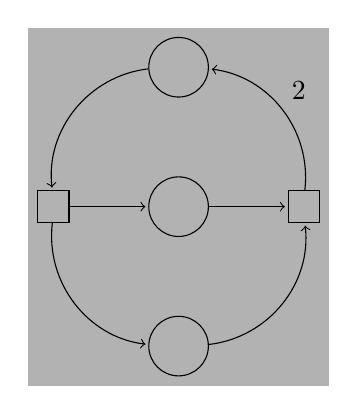
\begin{tikzpicture}[bend angle=45]
  \node[place]      (waiting)                            {};
  \node[place]      (critical)       [below=of waiting]  {};
  \node[place]      (semaphore)      [below=of critical] {};

  \node[transition] (leave critical) [right=of critical] {}
    edge [pre]                                 (critical)
    edge [post,bend right] node[auto,swap] {2} (waiting)
    edge [pre, bend left]                      (semaphore);
  \node[transition] (enter critical) [left=of critical]  {}
    edge [post]                                (critical)
    edge [pre, bend left]                      (waiting)
    edge [post,bend right]                     (semaphore);

  \begin{scope}[on background layer]
    \node [fill=black!30,fit=(waiting) (critical) (semaphore)
             (leave critical) (enter critical)] {};
  \end{scope}
\end{tikzpicture}
\end{codeexample}
}



\subsection{The Complete Code}

Hagen has now finally put everything together. Only then does he learn
that there is already a library for drawing Petri nets! It turns out
that this library mainly provides the same definitions as Hagen
did. For example, it defines a |place| style in a similar way as Hagen
did. Adjusting the code so that it uses the library shortens Hagen
code a bit, as shown in the following.

First, Hagen needs less style definitions, but he still needs to
specify the colors of places and transitions.

\begin{codeexample}[code only]
\begin{tikzpicture}
  [node distance=1.3cm,on grid,>=stealth',bend angle=45,auto,
   every place/.style=     {minimum size=6mm,thick,draw=blue!75,fill=blue!20},
   every transition/.style={thick,draw=black!75,fill=black!20},
   red place/.style=       {place,draw=red!75,fill=red!20},
   every label/.style=     {red}]
\end{codeexample}

Now comes the code for the nets:

{
\tikzset{%
  every place/.style={minimum size=6mm,thick,draw=blue!75,fill=blue!20},
  every transition/.style={thick,draw=black!75,fill=black!20},
  red place/.style={place,draw=red!75,fill=red!20},
  every label/.style={red},
  every picture/.style={on grid,node distance=1.3cm,>=stealth',bend angle=45,auto}}
\tikzexternaldisable
\begin{codeexample}[pre=\begin{tikzpicture},post=\end{tikzpicture}]
   \node [place,tokens=1] (w1)                                    {};
   \node [place]          (c1) [below=of w1]                      {};
   \node [place]          (s)  [below=of c1,label=above:$s\le 3$] {};
   \node [place]          (c2) [below=of s]                       {};
   \node [place,tokens=1] (w2) [below=of c2]                      {};

   \node [transition] (e1) [left=of c1] {}
     edge [pre,bend left]                  (w1)
     edge [post,bend right]                (s)
     edge [post]                           (c1);
   \node [transition] (e2) [left=of c2] {}
     edge [pre,bend right]                 (w2)
     edge [post,bend left]                 (s)
     edge [post]                           (c2);
   \node [transition] (l1) [right=of c1] {}
     edge [pre]                            (c1)
     edge [pre,bend left]                  (s)
     edge [post,bend right] node[swap] {2} (w1);
   \node [transition] (l2) [right=of c2] {}
     edge [pre]                            (c2)
     edge [pre,bend right]                 (s)
     edge [post,bend left]  node {2}       (w2);
\end{codeexample}
}

{
\tikzset{
every place/.style=     {minimum size=6mm,thick,draw=blue!75,fill=blue!20},
every transition/.style={thick,draw=black!75,fill=black!20},
red place/.style=  {place,draw=red!75,fill=red!20},
every label/.style={red},
every picture/.style={on grid,node distance=1.3cm,>=stealth',bend angle=45,auto}}
\tikzexternaldisable
\begin{codeexample}[pre=\begin{tikzpicture},post=\end{tikzpicture}]
  \begin{scope}[xshift=6cm]
    \node [place,tokens=1]     (w1')                            {};
    \node [place]              (c1') [below=of w1']             {};
    \node [red place]          (s1') [below=of c1',xshift=-5mm]
            [label=left:$s$]                                    {};
    \node [red place,tokens=3] (s2') [below=of c1',xshift=5mm]
            [label=right:$\bar s$]                              {};
    \node [place]              (c2') [below=of s1',xshift=5mm]  {};
    \node [place,tokens=1]     (w2') [below=of c2']             {};

    \node [transition] (e1') [left=of c1'] {}
      edge [pre,bend left]                  (w1')
      edge [post]                           (s1')
      edge [pre]                            (s2')
      edge [post]                           (c1');
    \node [transition] (e2') [left=of c2'] {}
      edge [pre,bend right]                 (w2')
      edge [post]                           (s1')
      edge [pre]                            (s2')
      edge [post]                           (c2');
    \node [transition] (l1') [right=of c1'] {}
      edge [pre]                            (c1')
      edge [pre]                            (s1')
      edge [post]                           (s2')
      edge [post,bend right] node[swap] {2} (w1');
    \node [transition] (l2') [right=of c2'] {}
      edge [pre]                            (c2')
      edge [pre]                            (s1')
      edge [post]                           (s2')
      edge [post,bend left]  node {2}       (w2');
  \end{scope}
\end{codeexample}
}

The code for the background and the snake is the following:

\begin{codeexample}[code only]
  \begin{scope}[on background layer]
    \node (r1) [fill=black!10,rounded corners,fit=(w1)(w2)(e1)(e2)(l1)(l2)] {};
    \node (r2) [fill=black!10,rounded corners,fit=(w1')(w2')(e1')(e2')(l1')(l2')] {};
  \end{scope}

  \draw [shorten >=1mm,-to,thick,decorate,
         decoration={snake,amplitude=.4mm,segment length=2mm,
                     pre=moveto,pre length=1mm,post length=2mm}]
    (r1) -- (r2) node [above=1mm,midway,text width=3cm,align=center]
      {replacement of the \textcolor{red}{capacity} by \textcolor{red}{two places}};
\end{tikzpicture}
\end{codeexample}
